\documentclass[letterpaper,inpress]{jdsart}

\setcounter{page}{1}
\pubmonth{July}
\pubyear{2020}
\volume{xx}
\issue{xx}
\doi{0000}


\usepackage[utf8]{inputenc}
\providecommand{\tightlist}{%
  \setlength{\itemsep}{0pt}\setlength{\parskip}{0pt}}


\usepackage{amsfonts,amsmath,amssymb,amsthm} \usepackage{booktabs} \usepackage{lipsum} \newcommand{\db}[1]{{\textcolor{blue}{#1}}} \newcommand{\svp}[1]{{\textcolor{red}{#1}}}

\begin{document}
\begin{frontmatter}

\title{Exploring Rural Shrink Smart Through Guided Discovery Dashboards}


\author[1]{
  \inits{D.}
  \fnms{Denise}
  \snm{Bradford}  \thanksref{1}  \ead{denise.bradford@huskers.unl.edu}}
\author[1]{
  \inits{S.}
  \fnms{Susan}
  \snm{VanderPlas}  \thanksref{1}}

\thankstext[type=corresp,id=1]{Corresponding author}
\address[1]{Department of Statistics, 
  \institution{University of Nebraska - Lincoln}, \cny{United States of America}}

\begin{abstract}
Many small and rural places are shrinking. Interactive dashboards are the most common use cases for data visualization and context for exploratory data tools. In our paper, we will explore the specific scope of how dashboards are used in small and rural area to empower novice analysts to make data-driven decisions. Our framework will suggest a number of research directions to better support small and rural places from shrinking using an interactive dashboard design, implementation and use for the every day analyst.
\end{abstract}

\begin{keywords}
\kwd{Interactive Dashboards}\kwd{Exploratory Data Analysis (EDA)}\kwd{Parallel Coordinate Plots (PCP)}\kwd{Guided Discovery Learning (GDL)}.
\end{keywords}

\end{frontmatter}

\hypertarget{abstract}{%
\section{Abstract}\label{abstract}}

Many small and rural places are shrinking. Interactive dashboards are the most common use cases for data visualization and context for exploratory data tools. In our paper, we will explore the specific scope of how dashboards are used in small and rural area to empower novice analysts to make data-driven decisions. Our framework will suggest a number of research directions to better support small and rural places from shrinking using an interactive dashboard design, implementation and use for the every day analyst.

\hypertarget{introduction}{%
\section{Introduction}\label{introduction}}

{\textcolor{red}{As the amount of data has increased in nearly every facet of life, the need to make sense of that data in an approachable, accessible form has become ever more important. 
As a result, many companies and organizations use interactive dashboards to present these data in a more useful and visually appealing form \citep{fisher}.}}

{\textcolor{red}{In many cases, dashboards support viewers' information processing, helping to make sense of complex data, navigate through a dataset, and supporting decision making based on the data.}}

{\textcolor{red}{Dashboards are often used, as with the car display of the same name, to provide summary information about many separate attributes of a common entity. One glance at a car's dashboard will tell you the speed, RPM, engine temperature, amount of gas in the tank; more importantly, however, the goal is not for the user to remember all of these characteristics, but to assess whether any of these quantities is outside of the expected range. 
Similarly, interactive dashboards for data are often used to display many different attributes and performance metrics which are of importance for stakeholders.}}

{\textcolor{red}{In this paper, we discuss the process of designing a dashboard to present publicly available government data to stakeholders in small Iowa towns to facilitate decision making and objective comparison with other similarly-situated towns.}}

Some communities continue to thrive as they lose population because they adapt, maintaining quality of life and community services for residents while investing in the future.
This process, \emph{smart shrinkage}, is important for rural areas who have experienced shrinking populations for decades.
As small rural towns do not have access to data scientists or even the ability to easily leverage data collected locally to support decisions, our research team will provide communities with data about services in small town Iowa in order to assist with developing strategies to improve quality of life for their residents amid shrinking populations \citep{scc}.
We hope to allow towns to discover their own data and compare to other similar towns, centering decision-making on data in the context of small-town Iowa life.
In the process, we will assess our visualizations to determine which strategies for user interface and interactive graphics design are most useful to empower town leaders to make discoveries in publicly available data assembled with a focus on items that impact rural quality of life.
{\textcolor{red}{This paragraph is pretty good, but see if you can tweak it to blend in a bit better with the edits I made above.}}

\section{Data Description}

Data collected from \url{data.iowa.gov} were used to create the SCC dashboard. Most of these data sets are collected at a town/city or county {\textcolor{red}{spatial resolution, requiring us to carefully join data to ensure that these differences are respected while collating relevant information at the city level}}. {\textcolor{red}{In addition to the more commonly available statistics derived from e.g. the census and American Community Survey,}} \url{data.iowa.gov} contains {\textcolor{red}{several}} unique {\textcolor{red}{data sets}}, including local liquor sales, school building locations, town budgets and expenditures, hospital beds, Medicaid reimbursements, and other details that may provide information about local quality of life.

{\textcolor{red}{Data available on Iowa's data portal were augmented in some cases with higher-quality data sets in cases where the Iowa data were out of date or insufficiently accurate.}}

Data collected from ELSI from \url{https://nces.ed.gov} were used to show the distance to any private or public school. The National Center for Education Statistics (NCES) is the primary federal entity for collecting and analyzing data related to education.
{\textcolor{red}{Cite Dave's papers about the ISTP QOL metrics, including education}}

Data collected from the Index of Relative Rurality (IRR) {\textcolor{red}{Create a bibtex entry for this and cite it properly, please. Same goes for most of the other URLs.}} \url{https://www.ers.usda.gov/topics/rural-economy-population/rural-classifications/} were used in the SCC dashboard to help classify the towns. The Index of Relative Rurality (IRR) is a continuous, threshold-free, and unit-free measure of rurality. It is an alternative to the traditional discrete threshold-based classifications.The IRR ranges between 0 (low level of rurality, i.e., urban) and 1 (most rural). Four steps are involved in its design:

\begin{enumerate}
\item Identifying the dimensions of rurality: population size, density, remoteness, and built-up area.
\item Selecting measureable variables to adequately represent each dimension:
    \begin{itemize}
        \item Size: logarithm of population size
        \item Density: logarithm of population density.
        \item Remoteness: network distance.
        \item Built-up area: urban area (as defined by the US Census Bureau) as a percentage of total land area.
    \end{itemize}
\item Re-scaling the variables onto bounded scales that range from 0 to 1.
\item Selecting a link function: unweighted average of the four re-scaled variable.
\end{enumerate}

Data collected from Rural Urban Commuting Area Codes \texttt{usda} were used to help identify towns with commuting behaviors in our rural areas. The rural-urban commuting area (RUCA) codes classify U.S. census tracts using measures of population density, urbanization, and daily commuting. This data is on a zip code-level that will help identify those communities that commute to more urban areas. The most recent RUCA codes are based on data from the 2010 decennial census and the 2006-10 American Community Survey. The classification contains two levels. Whole numbers (1-10) delineate metropolitan, micropolitan, small town, and rural commuting areas based on the size and direction of the primary (largest) commuting flows.

One of the interesting features of this assembled data set is that missing data can be missing for multiple reasons: not all state data is complete, but data about certain services may also be missing because towns do not offer that service.
Thus, in addition to the usual challenges of working with real-world data that is ``messy'' in a variety of ways, we also have to contend with missing data that is missing due to the size of the community or the lack of services. This makes both visualization and statistical analysis more complicated.

\hypertarget{methods}{%
\section{Methods}\label{methods}}

\subsection{Identifying Key Metrics for our Dashboard Design}

\begin{center}
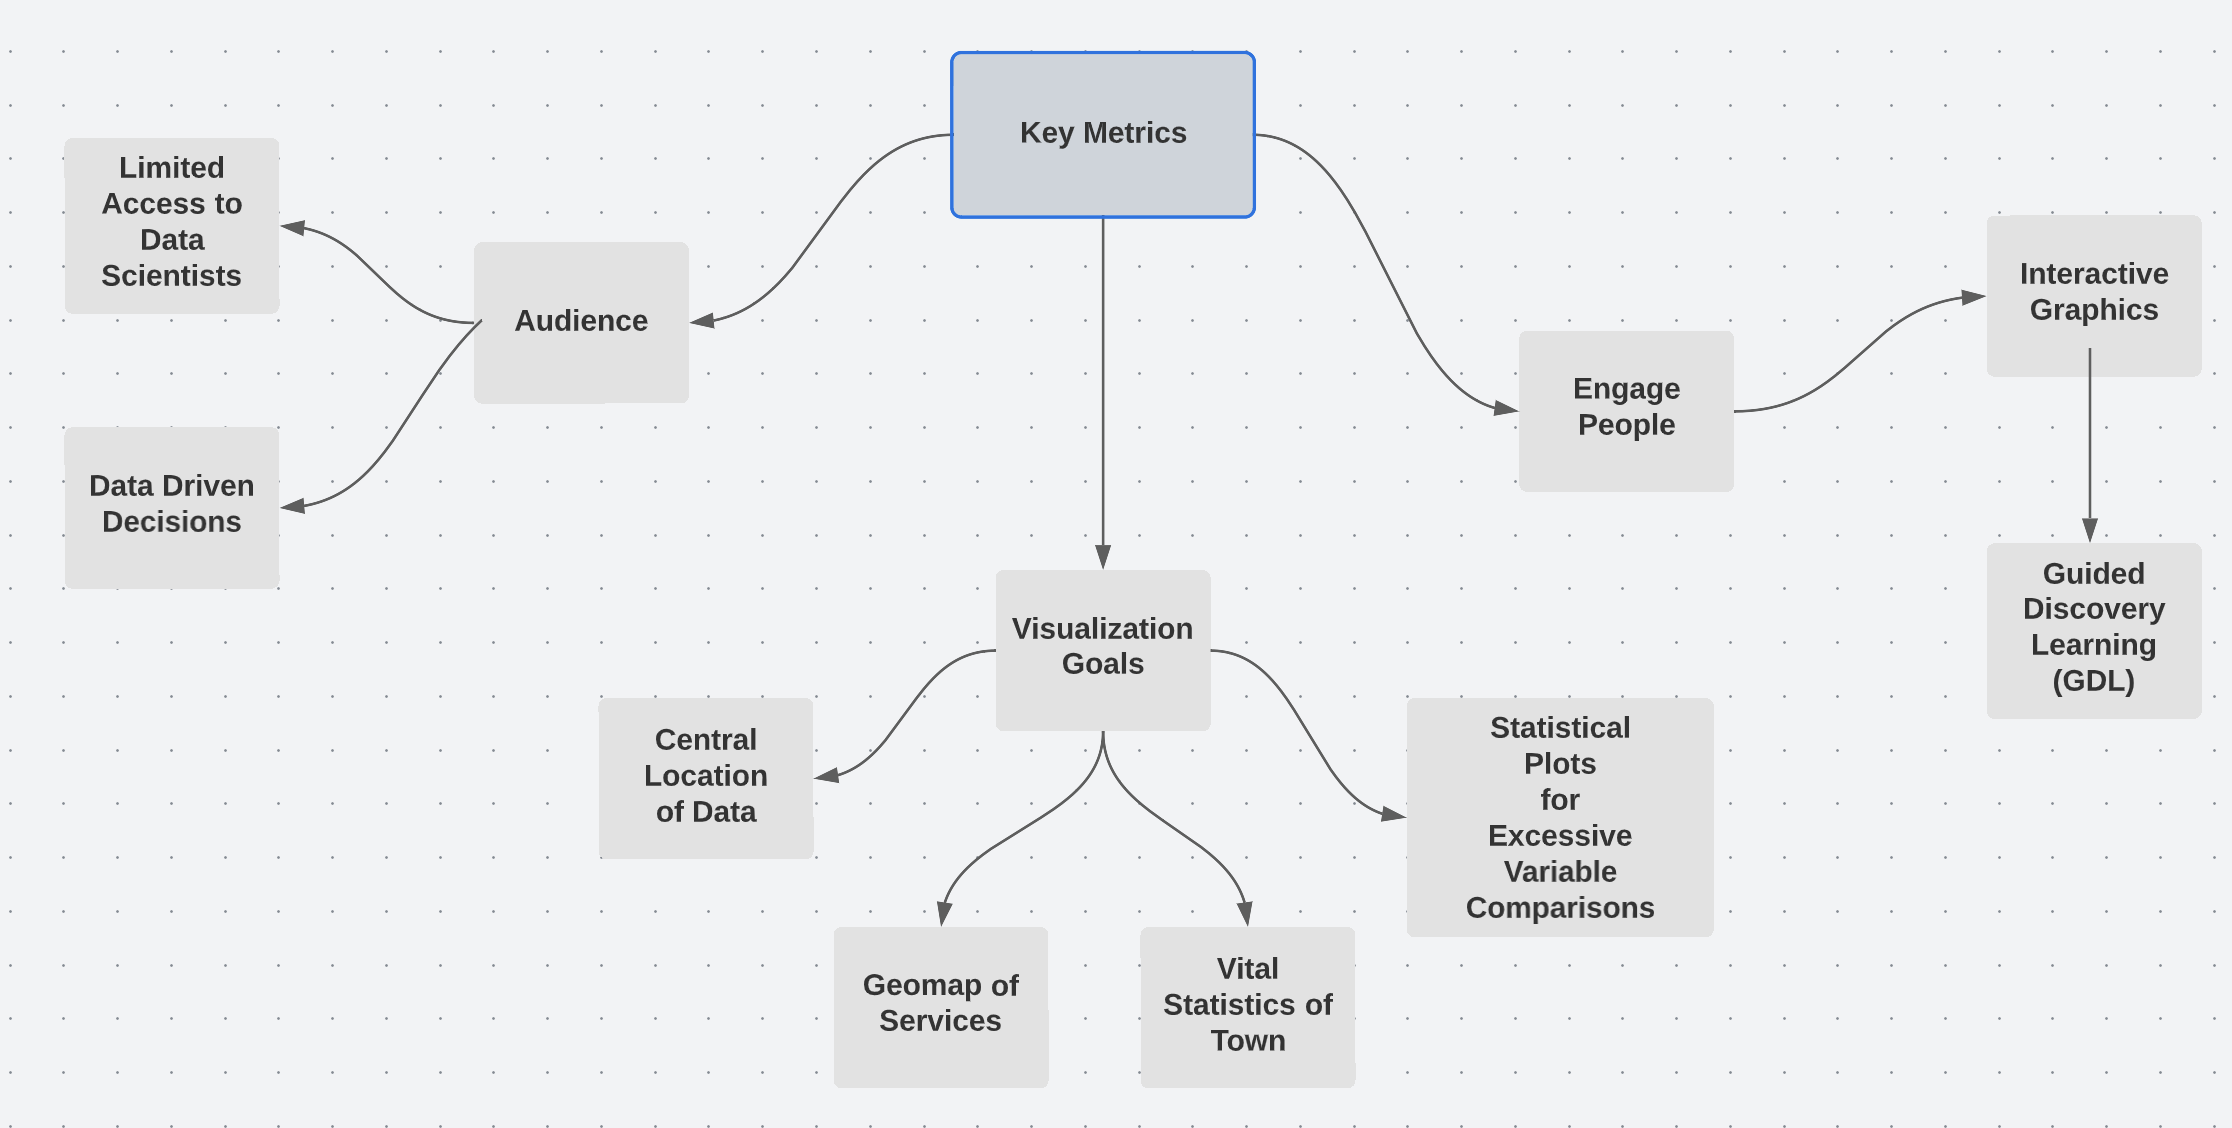
\includegraphics[width=.5\textwidth]{Key_Metrics}
\end{center}

{\textcolor{red}{One problem we identified early in the process of assessing smart-shrinkage strategies in small towns is that these towns do not have the resources to make data-driven decisions. Typically, small towns in Iowa are managed by at most a few part-time employees or volunteers. In some cases, essential management functions of the town are paid, but the municipalities we are interested in do not have sufficient funding to hire professionals to gather and analyze data.}}

{\textcolor{red}{As part of a wider project investigating the strategies towns use to maintain quality of life amid shrinking population, our research team provides communities with data about their own town, but also comparable towns across the state which may have a different approach to city services. In combination with other engagement strategies that are more qualitative, we hope to use this interactive dashboard approach to assist small Iowa cities with generalizing and developing strategies to improve or maintain quality of life amid shrinking populations.}}

{\textcolor{red}{One factor at the forefront of our visualization design is the importance of reducing the cognitive demands on viewers: we have assembled an incredible amount of data, and it is easy for even statisticians who deal with much larger datasets to get lost in the details of this data. At the same time, we want to invite viewers to engage with the data - to imagine, to draw comparisons, to generalize across towns, and to integrate outside information into the conclusions drawn based on the data we present.}}
{\textcolor{red}{Our initial strategy to accomplish this task is to utilize parallel coordinate plots (PCPs), a multivariate data visualization method that can accommodate both categorical and numerical data on in the same visualization. Supplementing the PCP that is the primary data display, we also provide some contextual information in the form of maps and "quick facts" that allow viewers to quickly assess a new town before comparing to a wider selection of towns.}}

We will assess our visualizations to determine which strategies for user interface and interactive graphics design are most useful to empower town leaders to make discoveries in publicly available data assembled with a focus on items that impact rural quality of life.

\subsection{Guiding Dashboard Design Principles}

An additional challenge is that research on dashboard creation and interactive visualization tends to be very task-specific and {\textcolor{red}{hard to apply to more generalized settings}}. That is, it is relatively easy to create a dashboard that works for a particular task, but it is hard to generalize from that process what will work for the next dashboard. With this in mind, we {\textcolor{red}{set out to clearly document our}} intentions at each stage of the design and evaluation process, with the goal of gathering some useful information about general dashboard design from the process of creating this specific dashboard.

Thus, our initial set of dashboard design principles is as follows:

\begin{itemize}
\item The town leaders are the focus audience; thus, the town itself should be the central focus of the app.
\item {\textcolor{red}{We should facilitate}} comparisons with other towns in order to allow the user to explore other potential solutions to offering services that enhance resident quality of life.
\item {\textcolor{red}{We will present}} the user with peer comparisons in order to widen the scope of exploration beyond the initial set of obvious peers in the local region.
\item {\textcolor{red}{We will implement feedback mechanisms that allow us to provide}} more detailed data and {\textcolor{red}{respond to}} feature requests to improve the dashboard design over time.
\end{itemize}

\subsection{Dashboard Design Process Overview}

We provided users with a town-centric approach: their town is at the center of our application, and comparisons to other, similar towns are secondary. As it can be extremely difficult to predict which towns are optimal for comparison purposes (similar may involve population, region, economic indicators, sports rivalries, and any number of other variables), we allow users to modify a set of suggested comparison towns to indicate other towns of interest. The suggested comparison towns are generated using unsupervised clustering methods on different sets of variables, but as we acknowledge that the problem of what towns should be used for comparisons is a tough one even for humans, we still want to allow for user input in this space. {\textcolor{red}{The initial design sketch and implementation are shown in}} \autoref{fig:v1}.

We {\textcolor{red}{implemented some suggested town comparisons using}} unsupervised clustering methods to help our towns make decisions that are informed in comparison to similar towns, for budget size, population size and location. {\textcolor{red}{We initially focused on}} determining the next five to ten similar towns, based on distances to services. We continue to use clustering methods to identify the towns that will be best compared when the analyst interacts with our dashboard. {\textcolor{red}{This feature became an important diagnostic for our data quality, but was not particularly useful to the application users, as they already know what towns they want to compare to; our suggested comparisons were just in the way.}}

{\textcolor{red}{We will conclude with an assessment of the initial layout design based on both direct user feedback through the survey form and based on UI clicks that provide a passive feedback mechanism to indicate what elements of the UI the users tend to interact with. We will also discuss verbal feedback we received when testing the application.}}

{\textcolor{red}{As with many dashboards, this project is under continuous development; while it makes for an unsatisfactory conclusion, we do not have a "final" dashboard design because the application will continue to evolve. However, we have some useful insights into the process of creating an application designed to invite users to explore a large and complex dataset that we believe to be a useful contribution to work in this area.}}

\begin{figure}
\centering
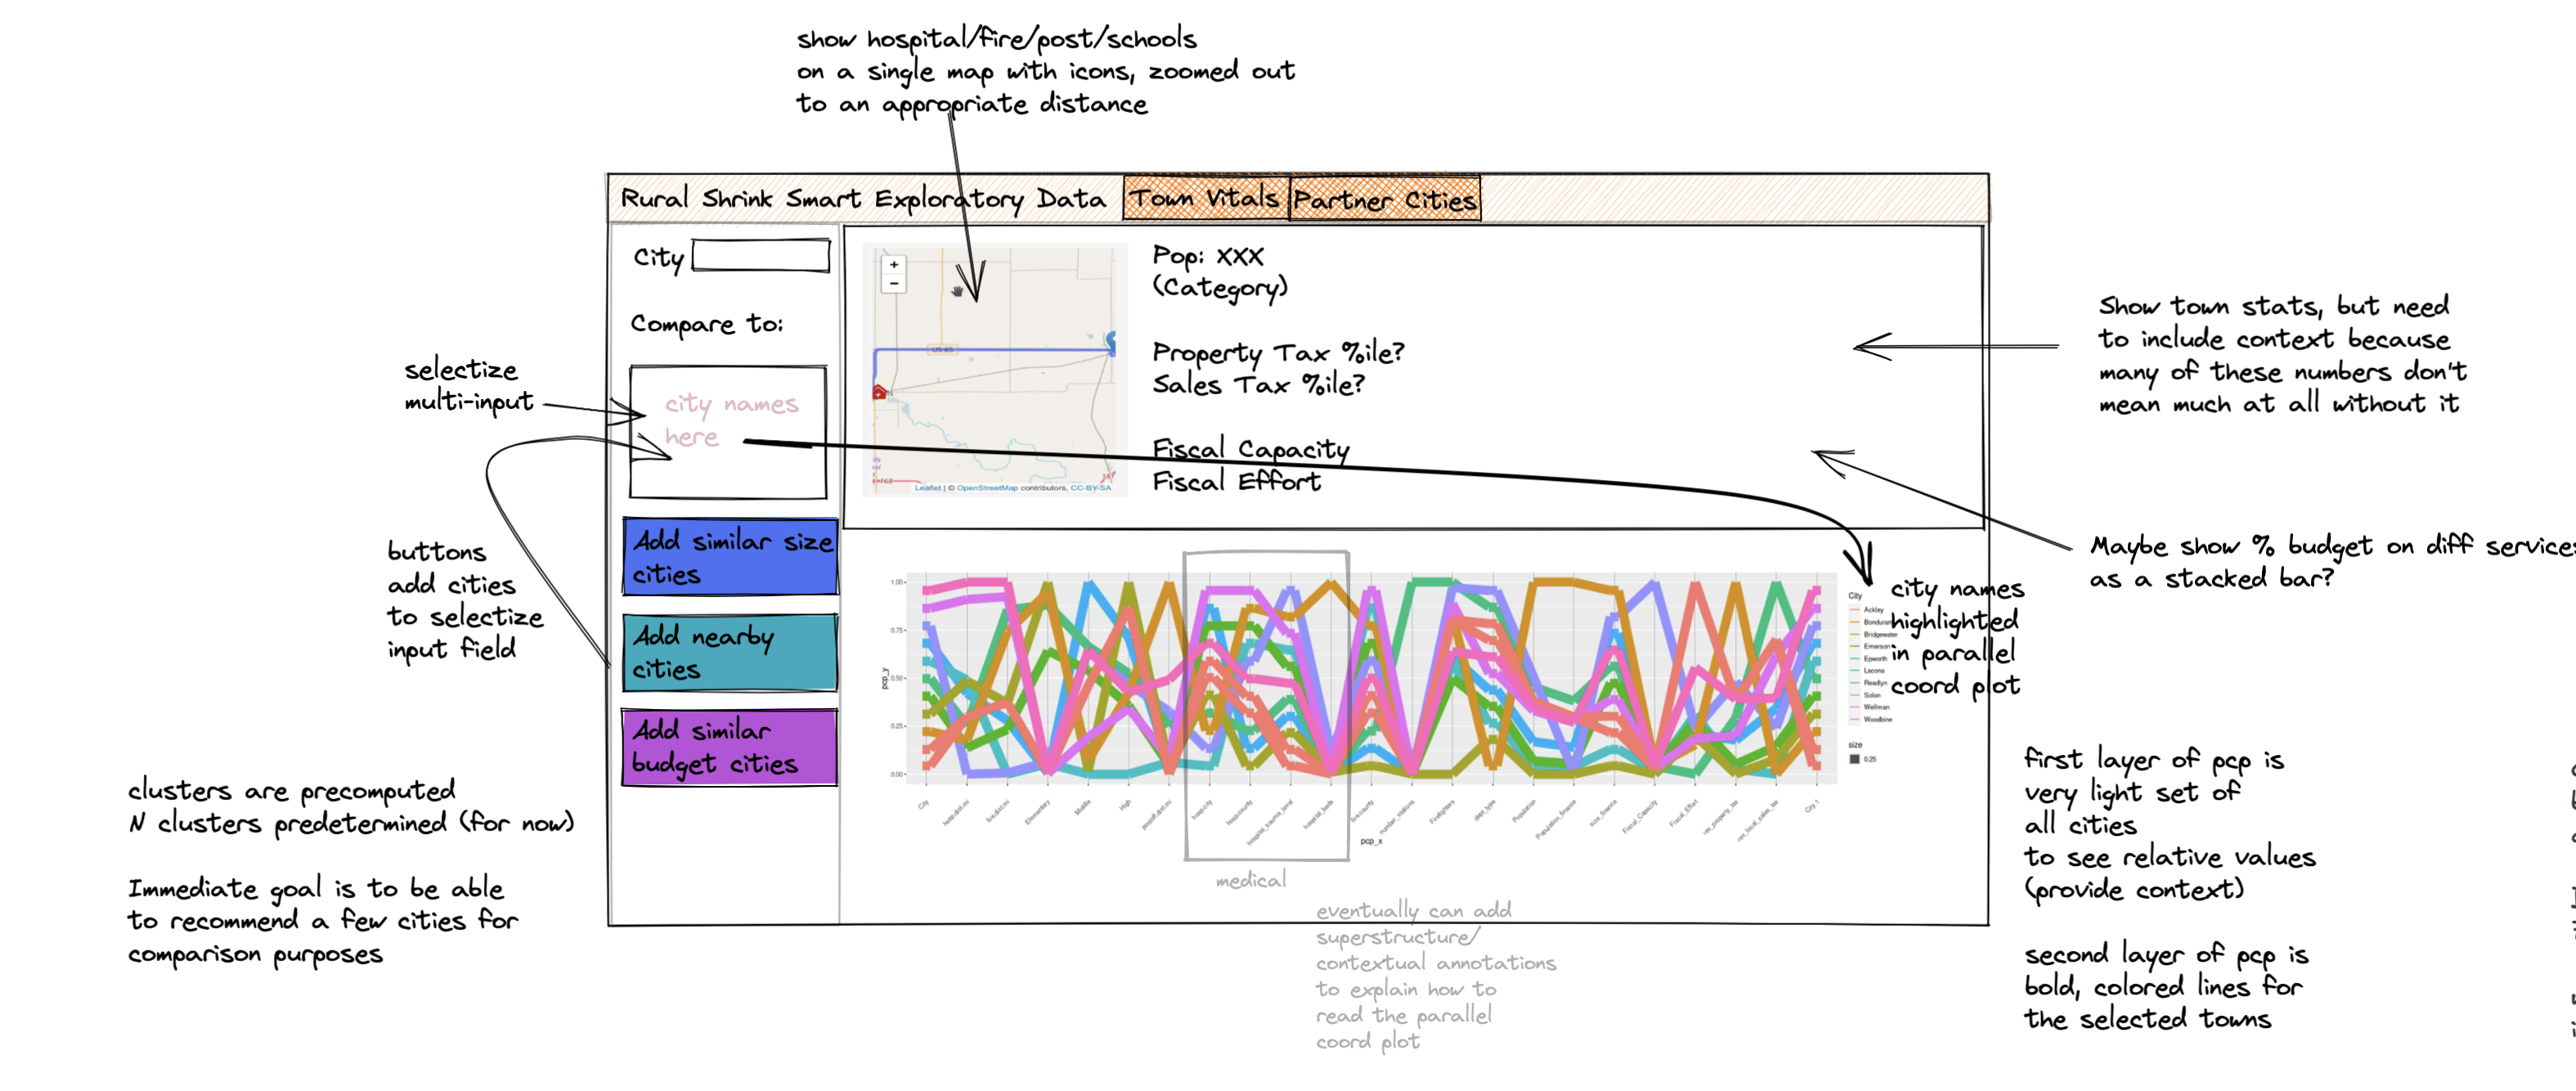
\includegraphics[width=\textwidth]{Version1}

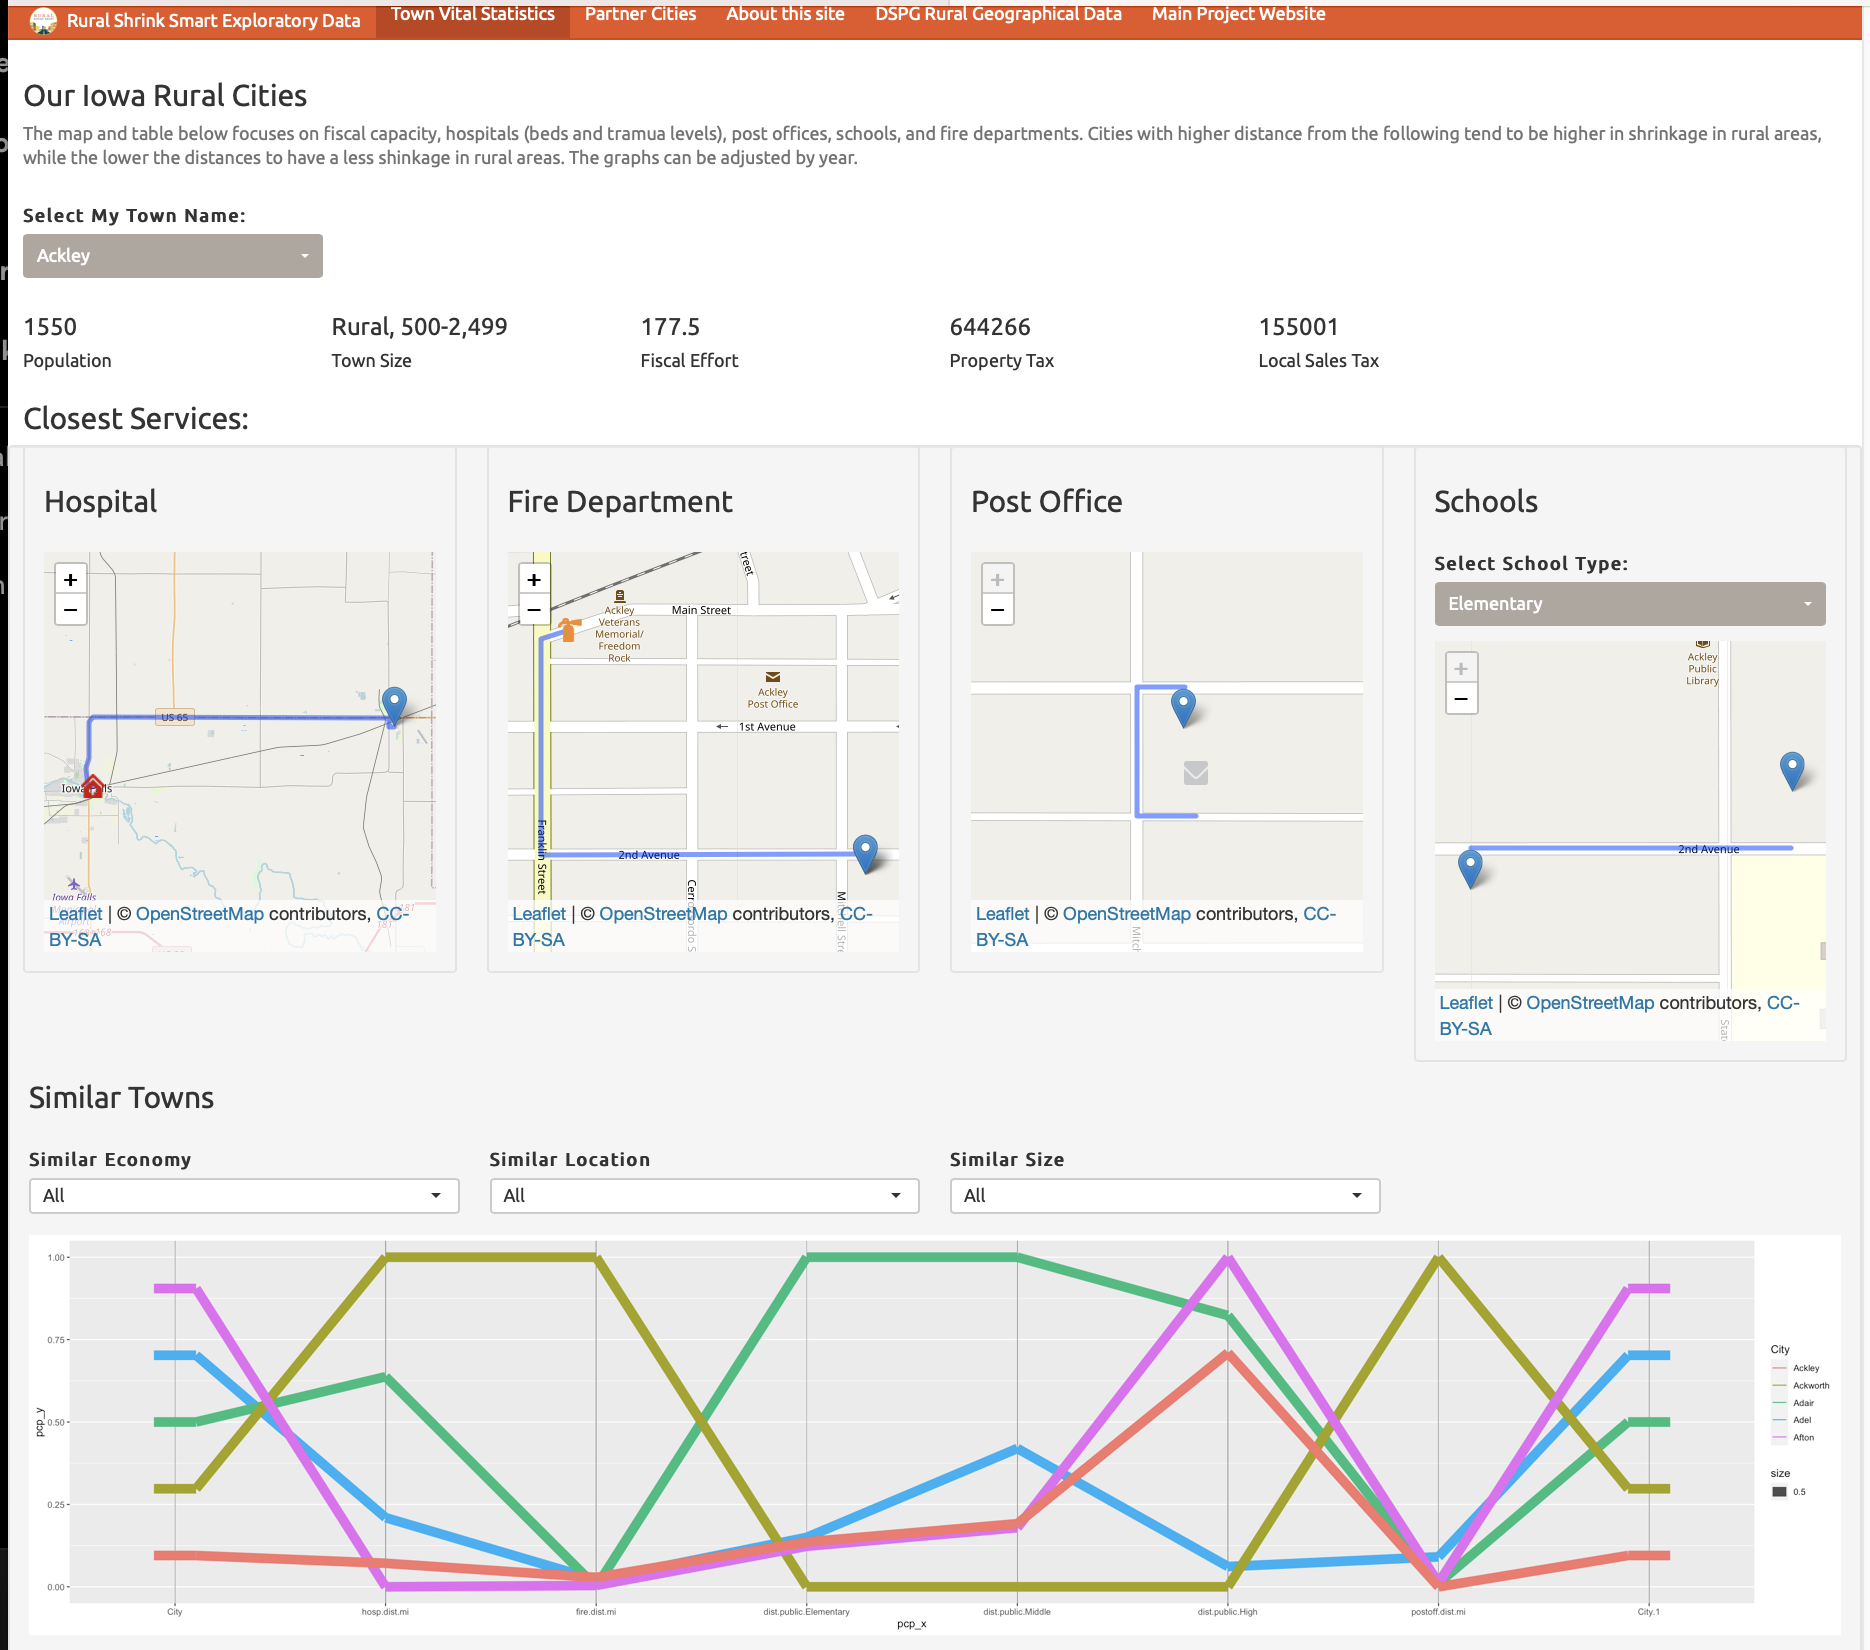
\includegraphics[width=.7\textwidth]{Version2}
\caption{Initial dashboard design sketch (top) and implementation (bottom).}\label{fig:v1}
\end{figure}

\begin{figure}
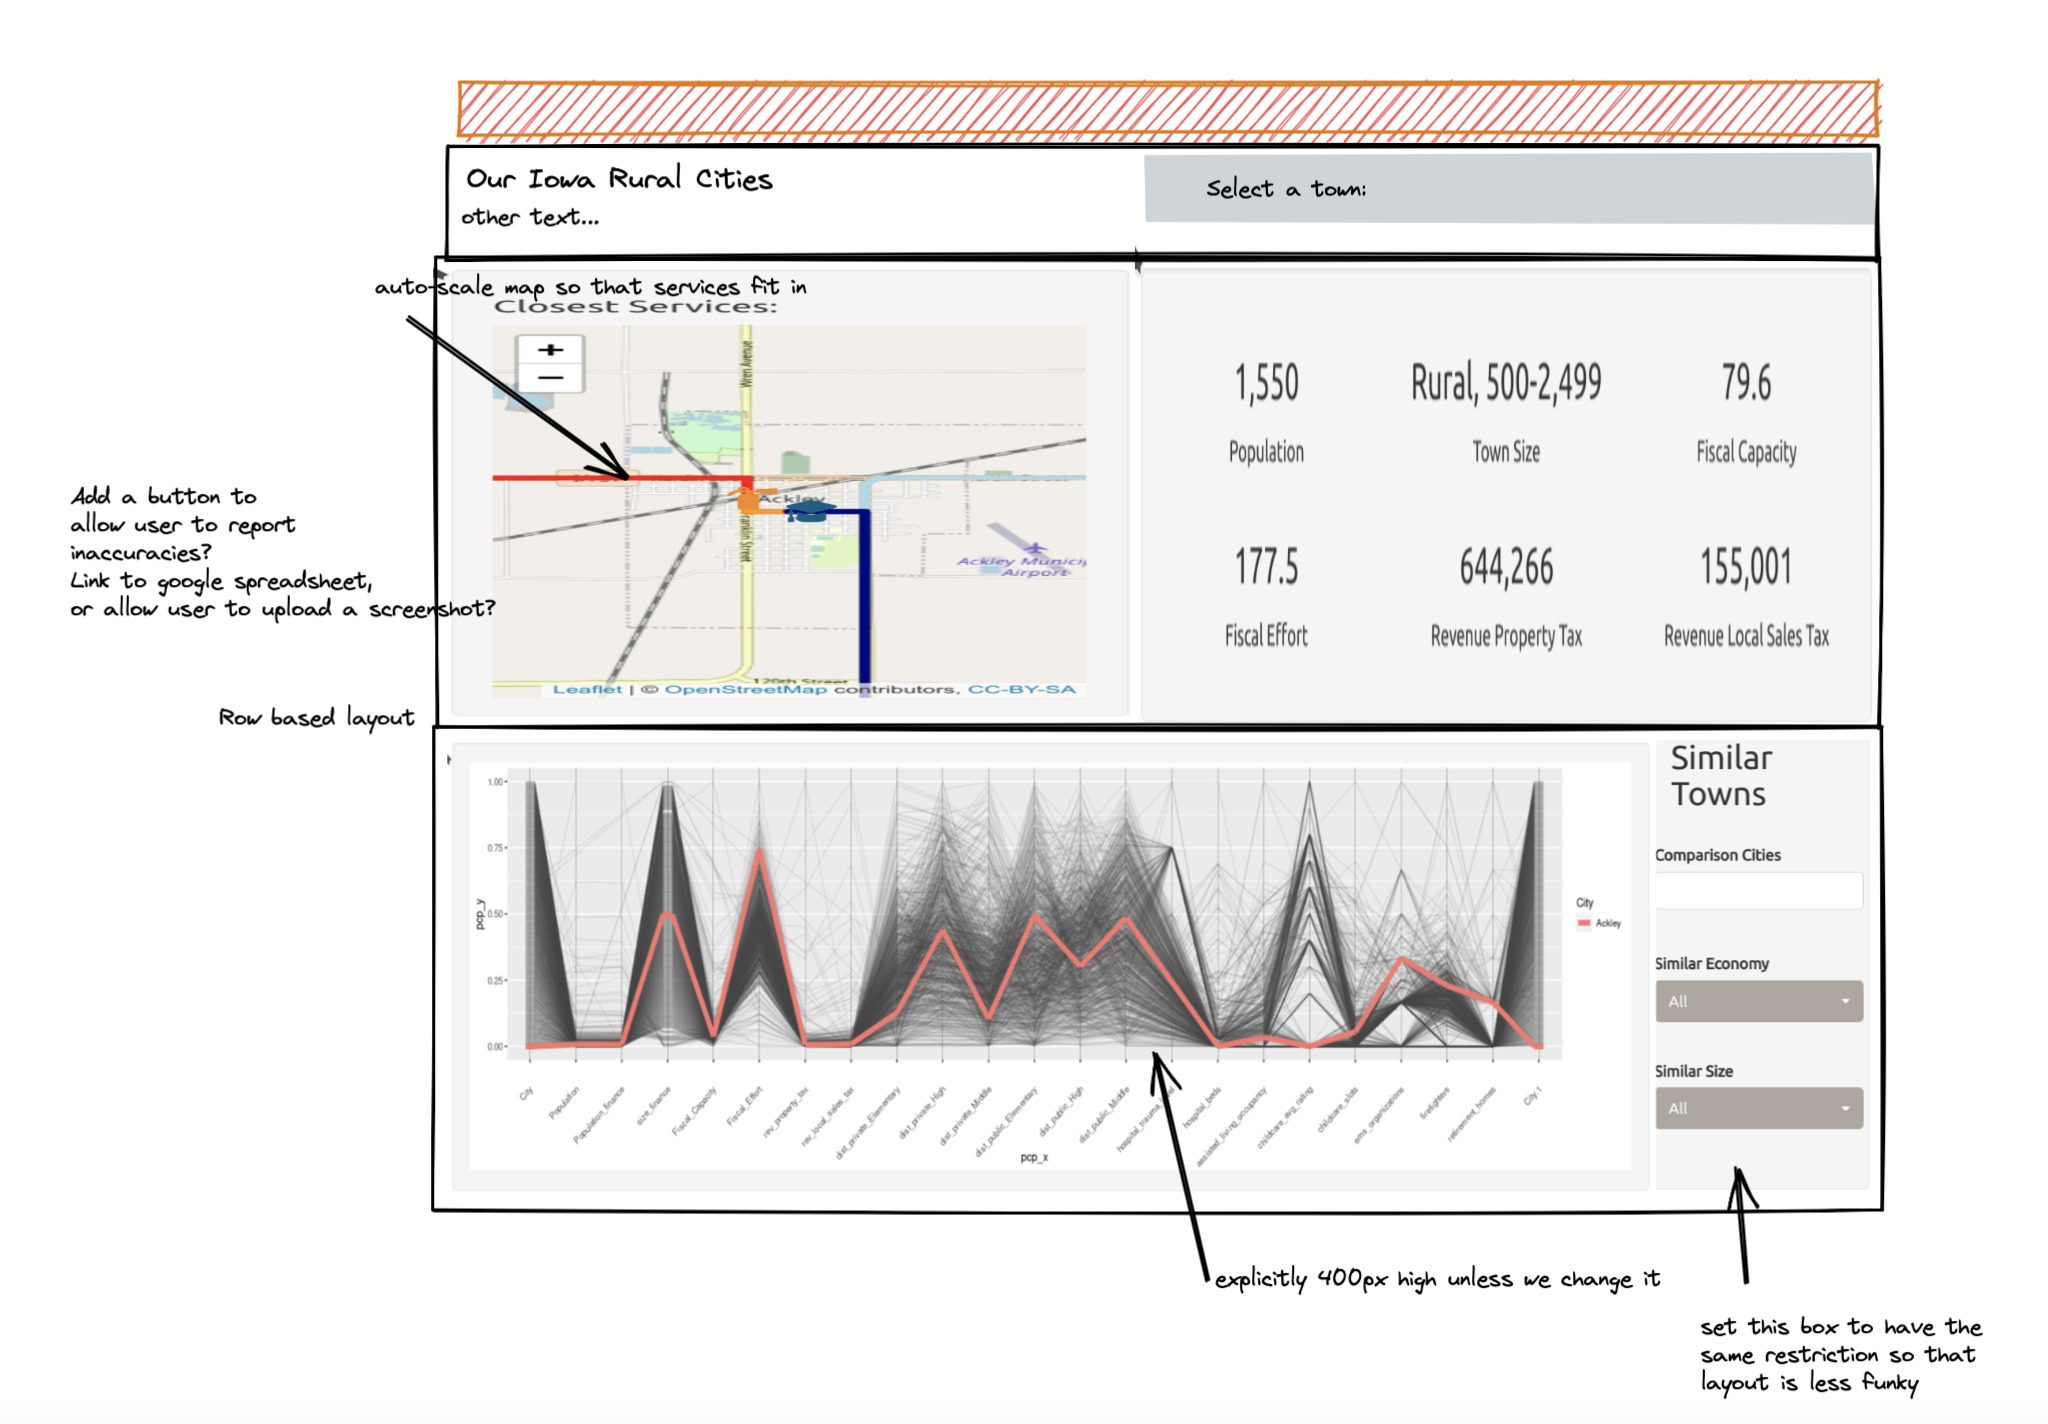
\includegraphics[width=.8\textwidth]{Version3}

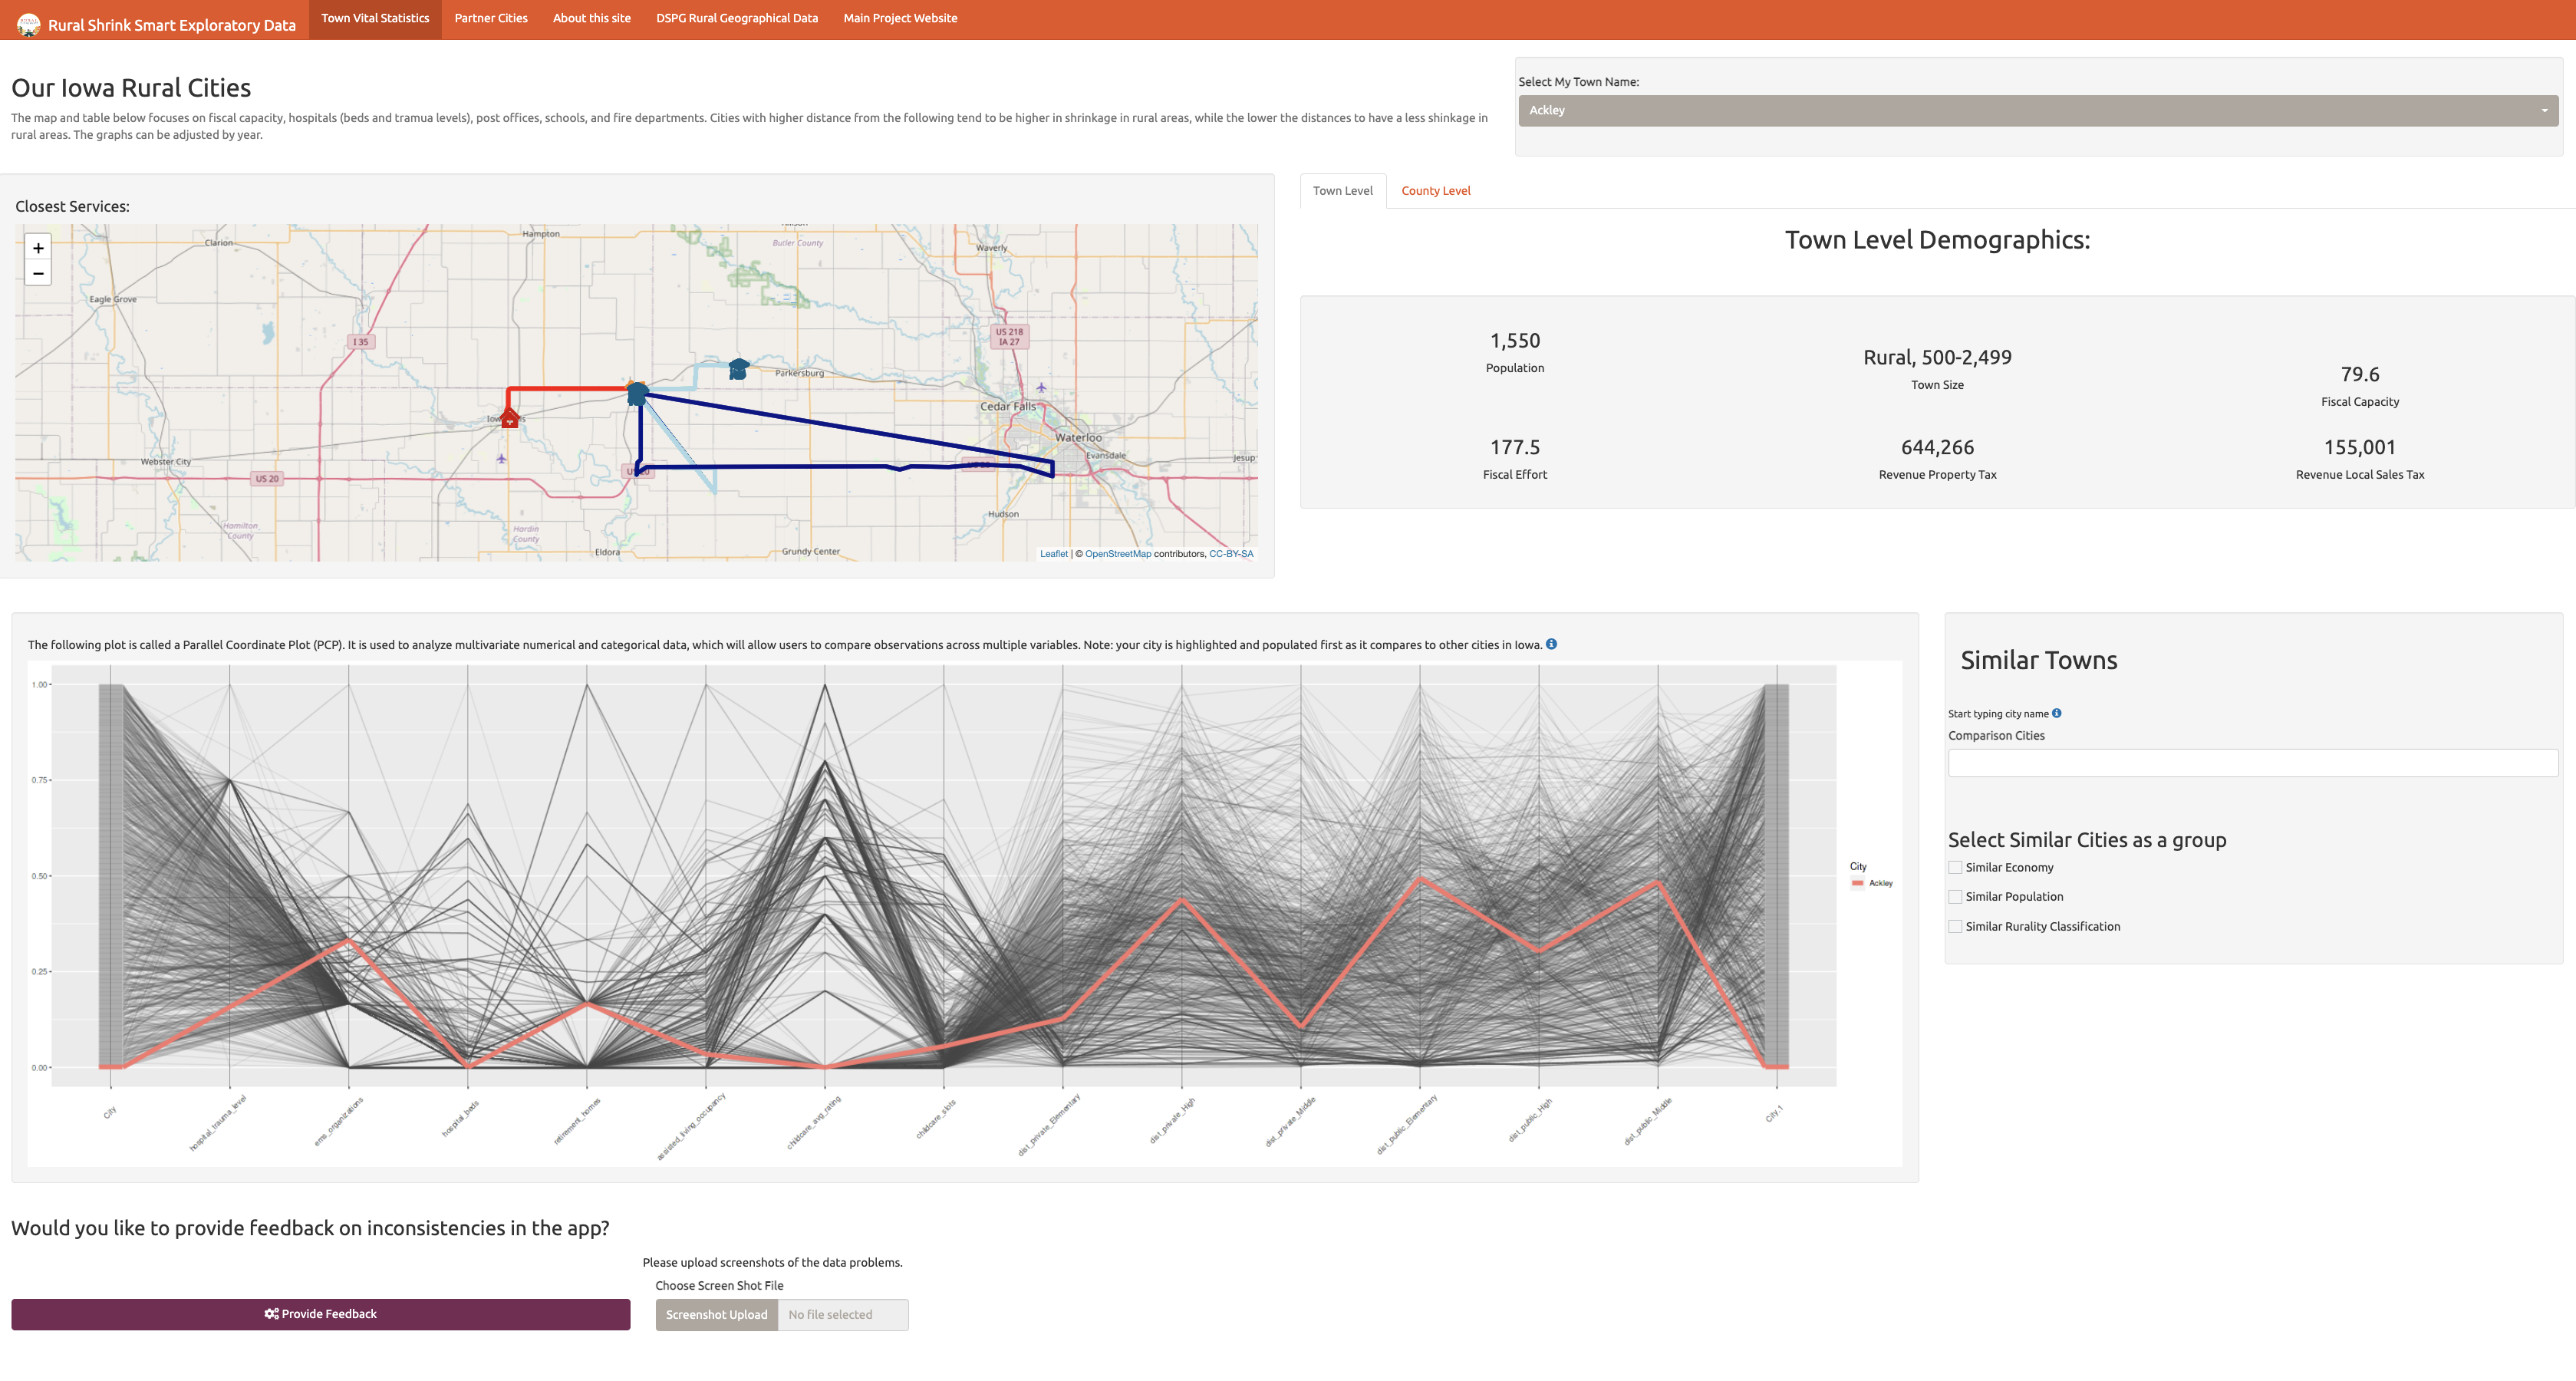
\includegraphics[width=\textwidth]{Version4}
\caption{A second iteration of the sketched design (top) and the implementation (bottom).}\label{fig:v2}
\end{figure}

\subsubsection{Dashboard Components}

The large set of publicly available data (primarily from \url{data.iowa.gov}) we have assembled is useful, but we must be careful with how we present this data because it would be easy to overwhelm the user with small details that mask the bigger picture. We select a small subset of towns (out of the 999 towns in Iowa) and a small subset of variables of interest to start with, and then allow the user to increase the complexity of the display in accordance with their interest. This avoids some of the pitfalls of dashboard design that can easily lead to user overload \texttt{few}.

While our dashboard layout is vitally important into making sure that the town leaders are using the dashboards, we should discuss the dashboard components that we used along with the philosophy of those key components. Starting with our parallel coordinate plot, which will allow for objective measures related to the QoL Survey. As our primary objective is to provide users with a town-centric approach: their town is at the center of our application, and comparisons to other, similar towns are secondary. We believe that this will allow the town leaders the ability to see as much data as possible with relation to their towns and others. The framework mentioned in \texttt{lee},``How do People Make Sense of Unfamiliar Visualizations?: A Grounded Model of Novice's Information Visualization Sensemaking,'\,' allowed our work to determine that a novice user seeing a PCP will be able to determine two basic components: Visual Object (textual objects and non-textual objects) and Frame (frame of content and frame of visual encoding). The PCP in this study were found to be promising for novice users, when comparing to the Treemap and Chord Diagram.

Furthermore, the large set of publicly available data we have assembled is useful, but we must be careful with how we present this data because it would be easy to overwhelm the user with small details that mask the bigger picture.

\subsection{Guided Discovery Learning (GDL)}

We leverage the framework of Guided Discovery Learning (GDL) to guide the town leaders to make discoveries using our interactive visualization. This framework leverages hints, feedback, and other helpful information to guide users in interactive exploration \texttt{dedonno}.

The Data Visualization component with GDL principles is a single page which populates the information in maps related to necessary services, including directions and distance to the fire department, schools, post offices, and hospitals. Value Boxes populate vital statistics sections that have information about the town's QoL Metrics and financial metrics, followed by a parallel coordinate plot that allows the town to see five towns that are similarly based on the most common variables in the towns, such as similar economy or population size. The graphical representations including a parallel coordinate plot and geographic maps {[}Figure 1{]}. The Rural Smart EDA Dashboard map visuals were built using OSRM route functions in R to amplify the accuracy of the distances from necessary services in town-centric point.

The Exploratory Data Analysis component utilizing statistical clustering methods enables the town leaders to interact with the parallel coordinate plots at various levels of granularities of data, with constraints, to similar towns. The Rural Smart EDA Dashboard features offer geospatial and structural data to assist town leaders in gaining a comprehensive understanding of the town in which they support.

Each component provides the town leaders with analytical aspects related to the performance of their town. As town leaders interact with the tool more helps build the knowledge and understanding different dimensions and measures related to the shrinkage of the town to a particular indicator.

\subsection{User Testing}

In this paper, we present the results from testing this application with users, and examine the implications for the feedback we received on our application design and on the more general design of dashboards for statistical novices. We examine which aspects of dashboard design ``common knowledge'\,' hold up in practice, and assess why these principles may not hold in our use-case.

Complex visualizations are difficult to assess in vivo: it is fairly easy to design an experiment to test a single graphic, but much harder to test the interactive dashboards which consist of systems of displays and user interactions. As a result, it is important to continuously assess which ``common knowledge'\,' design principles stemming from more controlled experiments hold up in real-world situations.

Using the framework from ``Creating design guidelines for building city dashboards from a user's perspectives,'' \texttt{young}, we will help summarize a users concerns utilizing six main critiques, which are framed into questions. We will adapt these questions to better help the town leaders communicate clear feedback for our team to use. We will collect how the users are experiencing the app with these set questions:

\begin{itemize}
\item Is the information the dashboard presents clear? \textit{(Scope)}
\item Is the dashboard easy to navigate? \textit{(Usability)}
\item Is the dashboard used in a socially responsible manner? \textit{(Ethics)}
\item Do you believe that you can trust the Rural Shrink Smart dashboard? \textit{(Validity)}
\item Do you find value in the Rural Shrink Smart dashboard? \textit{(Utility)}
\end{itemize}

\subsubsection{Beta Testing}

Our Beta testing of a design dashboard before deploying the product to our town leaders, we allowed users from the following groups:

\begin{itemize}
    \item Graphics Group Members (Users know Statistical Graphics)
    \item Rural Shrink Smart Project Members (Users know the project with little background in Statistical Graphics)
    \item  Others (Member of doctoral community that has background in educational adaptivity)
\end{itemize}

While this may not be a large sample size, our range of testers helped with changing approaches in data collection and dashboard changes.

\section{Discussion and Future Research}

\subsection{Data Collection Revisited}

As mentioned above, we wanted to use Unsupervised Clustering Methods to determine similar towns, however we were able to use this methodology to determine data quality in our open data sources. This work empowered our time to look for other open data sources to validate our vital statistics and maps. Since the clustering methods were used differently, we decided to use the USDA's version of rural area definitions. This allowed for a more transparent look into towns that may be similar based on there rurality index. Similar to the Census, the rurality metrics are county based and updated every ten years. This could later cause a problem for towns that may be shrinking faster than the collection of data. It could be worth looking into developing a proxy from our data collected that would be reliable for the years in between the USDA's collected years.

In a related idea of making sure that the towns are identified correctly, we should look into the aging of our towns. This may be important to identify the reasons for shrinking. In the event, that the towns are aging, will we be able to identify how fast the younger generation is moving out of the towns. This could be the most important piece of truly identifying the use of data in towns with an aging population.

\subsection{Visualization Revisited}

In our statistical graphs, we used Parallel Coordinate Plots (PCPs) to allow the user to look at a variety of variables, while the Guided Discovery Learning was used to makes sure that the users were informed of the information that was presented, it did not allow for the town leaders any more ease in understanding. As a result, we decided to look for easier ways to display data, such as boxplots and barplots. This direction will be limited but may be useful foor the sake of ease on the town leaders.

In the event that we want to continue to have the town leaders explore using a different statistical graphic, we would like to introduce the flower plot. This method may not represent that data in the way that could be misleading for understanding, we believe that the flower plot will allow for town leaders to engage in being curious as they explore more dimensions of data related to their Quality of Life (QoL) survey.

\subsection{Feedback}

We will continue to engage with twon leaders to ensure that we are developing a product that will help them make better data-driven decisions that are useful to increasing their quality of life, which may lend itself to help less shrinkage in these rural areas.

\bibliography{jdsart-sample.bib}
\bibliographystyle{jds}


\end{document}
